\documentclass{article}

\usepackage{../preamble}
\standalonetrue

\pagestyle{fancy}
\fancyhf{}
\rhead{Section \thesection}
\lhead{PHYS 304 Lecture 2}
\rfoot{Page \thepage}


\title{PHYS 304 Lecture 2}
\author{Ashtan Mistal}
\date{!!!}

\begin{document}

\ifstandalone
\maketitle
\fi

\graphicspath{{./Lecture02/}}

\section{Introduction}


\subsection{Review of key points from last day}

Quantum mechanics is mysterious, in large part due to the intrinsic uncertainty in a system’s behaviour, distinct from statistical or measurement uncertainties.

Waves are distributed displacements of some quantity in space and time.

Pure waves have well-defined wavelengths and periods, or frequencies.

Interference, or the superposition of distinct distributed displacements, in some sense defines “wavelike behaviour”.

The Bach paper that was for pre-reading describes experiments where diffraction patterns are observed on electron detector screens that record individual electron arrivals, when averaged over a long time (many many electrons incident on the electron-double slit.  


\subsection{Today's activities}

\begin{itemize}
    \item Review and reflect on how a classical particle kinetics problem is solved.
    \item Introduce the fundamental postulates of the quantum mechanical approach to solving particle kinetic problems.
    \item Contrast the two approaches, from both mathematical and conceptual perspectives.
\end{itemize}

\section{One-Dimensional Quantum Mechanics}

Use a particle moving in 1 dimension in a time-independent potential as the basis for learning how to treat an object quantum mechanically. 

Remind yourselves how to classically solve for the motion of a particle with mass m travelling in the positive x direction with a speed of 100 m/s if it was at position x=0 at time t=0, and there is a uniform electric field exerting a force on the electron of 1 N in the negative x direction.

Think on your own, and in pairs for a couple of minutes. (Think, Pair, Share (TPS))

\begin{itemize}
    \item We went over the fully deterministic Newtonian equation of motion.
\end{itemize}

Firstly, let us start with Newton's law of motion:

$$F = ma$$

$$d \frac{d^2 x(t)}{dt^2} = F = -qE = \text{constant}$$

$$\frac{dx}{dt} = \frac{F}{m} t + c_1$$

$$x(t) = \frac{F}{2m} t^2 + c_1 t + c_2$$

$$x(0) = 0 \Rightarrow c_2 = 0$$

$$v(0) = 0 \Rightarrow c_1 = v_0$$

$$\Rightarrow x(t) = v_0 t - \frac{qE}{2m} t^2$$

Implicitly, $x$ represents the center of mass of the particle, which doesn't chance size or shape, and explicitly, $x = x(t)$: the center of mass of the particle depends on time, and that the solution describes. 

\subsection{Activity 2}

In Quantum Mechanics, in contrast to solving equations for $x(t)$ directly, what does one have to find in order to calculate $x(t), v(t)$ etc. for the electron?  

The wavefunction of the electron: $\Psi(x,t)$

What is the differential equation “analogous to” $m \frac{d^2 x(t)}{dt^2} = F(x) = -\frac{d}{dx} V(x)$ one needs to solve to find the wavefunction?

$$i \hbar \frac{\partial \Psi}{\partial t} = - \frac{\hbar^2}{2m} \frac{\partial^2 \Psi}{\partial x^2} + V \Psi$$

How is the QM scenario operationally similar to the classical case?

\begin{itemize}
    \item A prescription for “deriving everything there can possibly be known about the particle’s future dynamics".
\end{itemize}

How is the QM scenario mathematically different from the classical case? (insert the arguments of the wavefunction and potential explicitly)  The “x” in Newton’s equation is entirely different from the “x” in Schrödinger’s equation!

What is the biggest difference between the two equations of motion, mathematically?

In QM, we have a partial differential equation for a quantity that depends on $x$ and $t$, versus an ordinary differential equation that depends only on $t$. 

Explicitly, write the implicit dependencies of $\Psi$ and $V$. What is the biggest difference conceptually?

\begin{itemize}
    \item $x$ is a parameter of $\Psi$, along with $t$, and it is not an explicit dynamical variable (the $x$ in this equation is not $x(t)$). 
\end{itemize}

\subsection{Activity 3}

\textit{important concept warning}

What connects the quantum mechanical wave function with the classical quantity x(t)?

$$\int_a^b |\Psi(x,t)|^2 dx = \left\{ \text{Probability of finding the particle between } a \text{ and } b \text{, at time } t \right\}$$

\begin{itemize}
    \item We sketched an electron "blob" in $\Psi^2(x,t)$ at two values of $t$. 
    \item We went through the case where localization was reasonably high, where it was "particle like", and where it was delocalized, or "wave-like". First the instance velocity has trivial connection to classical particle motion -- but what about the latter? It's more of a wave propagation velocity. 
    \item There is a large underlying uncertainty in psi itself, due to phase, so we're working with $\Psi^2$ for the time being. 
\end{itemize}

\subsection{Activity 4 and 5}

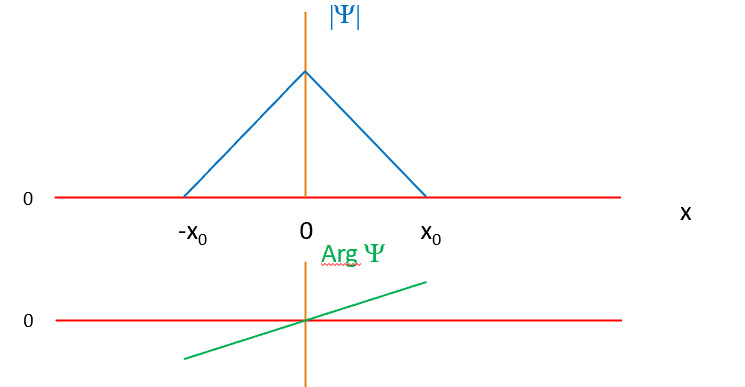
\includegraphics[width = 0.7 \textwidth]{Lecture02/1.png}

What is the most likely location you would measure an electron to be at $t = 1$s if $\Psi(x,t=1)$ was the above wavefunction?

\begin{itemize}
    \item Why aren't the $y$ axis values needed?
\end{itemize}

\subsection*{Activity 5}

How far away from that most likely position would finding the electron be half the most likely probability?

Firstly, we take the magnitude squared to get the probability distribution, and note that for $x > 0$, $|\Psi(x)| = |\Psi_{max}| (1 - \frac{x}{x_0})$. Note that $\Psi_{max}$ is when $x = 0$, the peak of the wavefunction.

\subsection{Activity 6}

What would be the consequence of performing a measurement and finding the particle at location x=c, to within some uncertainty dx?

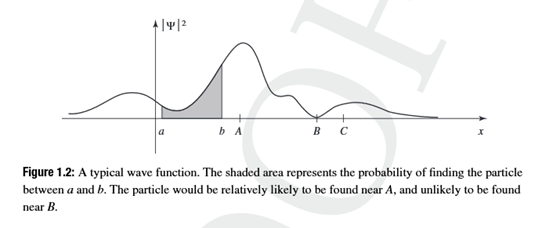
\includegraphics[width = 0.7 \textwidth]{Lecture02/2.png}

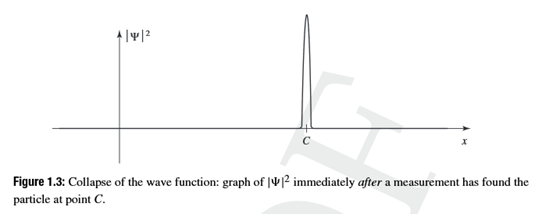
\includegraphics[width = 0.7 \textwidth]{Lecture02/3.png}

There is a lot of residual uncertainty in $\Psi$ itself (as noted above), due to the unknown phase. That would have to be determined from, a more detailed knowledge of how the "measurement" was performed. Note that a measurement is one of the most subtle aspects of quantum mechanics. 


\end{document}